\section[共振]{\makebox[5em][s]{共振}}\label{sec:07.05}

在有阻力的情况下,振子的振动是衰减的,因此,为了使阻
尼振子作不衰减的振动,必须时时给它补充能量。补充能量的一
种方式就是用外力作用到振子上,这时发生的运动,称为受迫振
动。扬声器中纸盆的振动,各种弦乐器中音腔薄木板随着琴弦的
振动,缝纽机中针的振动,蒸汽机活塞的振动等等,都属这类振
动。

在周期性外力作用下的振子,会产生一种特殊的效应,即所
谓共振。这是说,如果外力是周期性的,受迫振动有一类很特别
的现象,即共振。虽然周期性外力并不很大,但它所造成的振动
的振幅却特别大。

共振具有很重要的实用价值。无论在电学,光学等其他物理
学各部门中,或是在工程技术部门中,共振现象都是常遇到的。
下面我们来发展这一现象的理论。

受迫振动的物体受到三种力,即弹性力$ \left( - k x \right) $、阻力
$ \left( - \eta \dfrac { \dif x } { \dif t } \right) $
和周期性外力$ \left( F _ { 0 } \cos \omega t \right) $。所以,按照牛顿第二定律,有

~\vspace{-1.56em}
\begin{equation*}
  m \frac { \dif ^ { 2 } x } { \dif t ^ { 2 } } = - k x - \eta \frac { \dif x } { \dif t } + F _ { 0 } \cos \omega t
\end{equation*}
% 211.jpg

\clearpage
\begin{align*}
  \beforetext{或}\frac { \dif ^ { 2 } x } { \dif t ^ { 2 } } + \frac { \eta } { m } \cdot \frac { \dif x } { \dif t } + \frac { k } { m } x = \frac { F _ { 0 } } { m } \cos \omega t
\end{align*}
引入符号$ \omega _ { 0 } ^ { 2 } = \dfrac { k } { m } $,$ 2 \beta = \dfrac { \eta } { m } $,$ f _ { 0 } = \dfrac { F _ { 0 } } { m } $,则得
\begin{equation}\label{eqn:07.05.01}
  \frac { \dif ^ { 2 } x } { \dif t ^ { 2 } } + 2 \beta \frac { \dif x } { \dif t } + \omega _ { 0 } ^ { 2 } x = f _ { 0 } \cos \omega t
\end{equation}
这就是在周期性外力作用下,振子运动的基本方程。求它的一般
解比较繁,我们可以从物理角度判断一下运动的大致情况。如果
振动系统开始是静止的,则加上周期性外力后,应有很小的振动,
并渐渐加大,大到一定程度后,阻力的作用也增加,结果当阻力
所消耗的能量与外力所给予的能量相等时,振动就稳定下来。因
此,我们可以尝试一下去寻找稳定解,即具有下列形式的解:
\begin{equation}\label{eqn:07.05.02}
  x = A \cos \left( \omega ' t + \varphi _ { 0 } \right)
\end{equation}
将式\eqref{eqn:07.05.02}代入式\eqref{eqn:07.05.01},可以定出$ A $,$ \omega ' $,$ \varphi_{ 0 } $的值为
\begin{align}
  A               & = \frac { f _ { 0 } } { \sqrt { \left( \omega_{ 0 } ^ { 2 } - \omega ^ { 2 } \right) ^ { 2 } + 4 \beta ^ { 2 } \omega ^ { 2 } }} \label{eqn:07.05.03} \\
  \varphi _ { 0 } & = \tg ^ { - 1 } \frac { 2 \beta \omega } { \omega_{ 0 } ^ { 2 } - \omega ^ { 2 } } \label{eqn:07.05.04}                                               \\
  \omega '        & = \omega \label{eqn:07.05.05}
\end{align}
这就是稳定的受迫运动解。它描写了一个简谐振动,它的频
率等于周期性外力的频率。

解式\eqref{eqn:07.05.02}的一个最重要的特点是振幅$ A $和外力的频率有
关,而且,当$ \omega = \sqrt { \omega _ { 0 } ^ { 2 } - 2 \beta ^ { 2 } } $时,式\eqref{eqn:07.05.03}的分母达到极小,故
$ A $达到极大,这个$ \omega $称为共振频率。这就是说,当外力频率为共振
频率时,将引起最大的响应。由于$ \beta $一般很小,所以可近似地说,
当$ \omega \approx \omega _ { 0 } $时达到共振。

图\ref{fig:07.09}\;给出了$ A $作为$ \omega $的函数的曲线。这里所有曲线都有一个
峰,这就是共振。可以明显看到,如果振动系统的阻力越小,
% 212.jpg
\begin{wrapfigure}[8]{r}{16em}
  \centering
  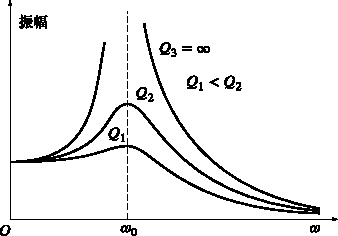
\includegraphics{figure/fig07.09}
  \caption{共振曲线}
  \label{fig:07.09}
\end{wrapfigure}
即品质因数$ Q $越大,则曲线的振幅峰越明显。也就是说,
系统的$ Q $值越大,则其共振现象越显著。

在极端情况,若阻力为零,即$ \beta = 0 $时,则
$ A = \dfrac { f _ { 0 } } { \left| \omega_{ 0 } ^ { 2 } - \omega ^ { 2 } \right| } $。
这时共振发生于$ \omega = \omega _ { 0 } $,而
且振幅无限大。而在
$ \omega \ne \omega _ { 0 } $时,$ A $具有有限值。

我们再从能量观点来分析一下受迫振动。在稳定振动时,质
点的振动振幅不变,也就是它的总机械能是不变的。但是,阻力
的存在随时消耗着振子的机械能。这说明周期性外力一定是在不
断地对谐振子作功,补偿了阻力的消耗。

既然外力供给振子的能量等于阻力消耗的能量,所以只要我
们计算出了后者,也就得到了前者。由式\eqref{eqn:07.04.05},阻力的功率为
$ \eta \left( \dfrac { \dif x } { \dif t } \right) ^ { 2 } $
,所以,平均每单位时间阻力所消耗的振子的能量为
\begin{equation}\label{eqn:07.05.06}
  \begin{aligned}
      & \frac { 1 } { T } \int _ { 0 } ^ { T } \eta \left( \frac { \dif x } { \dif t } \right) ^ { 2 } \dif t                                                              \\
    = & \frac { \eta f _ { 0 } ^ { 2 } \omega ^ { 2 } } { 2 \left[ \left( \omega_{ 0 } ^ { 2 } - \omega ^ { 2 } \right) ^ { 2 } + 4 \beta ^ { 2 } \omega ^ { 2 } \right] }
  \end{aligned}
\end{equation}
上式中$ T = \dfrac { 2 \uppi } { \omega } $的是振动周期。这种计算是把瞬时功率在一个周
期中进行平均。

式\eqref{eqn:07.05.06}就是平均每单位时间振子从外力吸取的能量,即平
均吸收功率。它表明,只当外力的频率$ \omega $接近谐振子的固有频率
% 213.jpg
$ \omega_{ 0 } $时,振子才能有效地吸收外力所提供的能量,而对其他频率的
外力所提供的能量,振子是很少吸收的。这种吸收具有选择性,
称为共振吸收。

如果阻力$ \beta $很小,$ \omega \approx \omega _ { 0 } $发生共振,由式\eqref{eqn:07.05.06}给出共振时
的吸收功率为
\begin{equation*}
  \frac { \eta f _ { 0 } ^ { 2 } } { 8 \beta ^ { 2 } } = \frac { m f _ { 0 } ^ { 2 } } { 4 \beta }
\end{equation*}
这里使用了$ \beta = \eta / 2 m $。当外力频率稍偏离$\omega_{ 0 }$时,吸收功率下降。
现在来求:吸收功率为上述极大值的一半时,外力频率$ \omega $与振子
的固有频率$ \omega_{ 0 } $差多少。即解方程
\begin{equation*}
  \frac { \eta f _ { 0 } ^ { 2 } } { 16 \beta ^ { 2 } } = \frac { \eta f _ { 0 } ^ { 2 } \omega ^ { 2 } } { 2 \left[ \left( \omega_{ 0 } ^ { 2 } - \omega ^ { 2 } \right) ^ { 2 } + 4 \beta ^ { 2 } \omega ^ { 2 } \right] }
\end{equation*}
采用$ \omega \approx \omega _ { 0 } $,则
\begin{equation*}
  \begin{aligned}
    \left( \omega _ { 0 } ^ { 2 } - \omega ^ { 2 } \right) & = \left( \omega _ { 0 } + \omega \right) \left( \omega _ { 0 } - \omega \right) \\
                                                           & \approx 2 \omega _ { 0 } \left( \omega _ { 0 } - \omega \right)
  \end{aligned}
\end{equation*}
\begin{align*}
  \beforetext{上式成为} & \frac { f _ { 0 } ^ { 2 } } { 16 \beta ^ { 2 } } = \frac { f _ { 0 } ^ { 2 } } { 2 \left[ 4 \left( \omega_{ 0 } - \omega \right) ^ { 2 } + 4 \beta ^ { 2 } \right] } \\
  \beforetext{解得}   & \left| \omega _ { 0 } - \omega \right| \approx \beta
\end{align*}
所以,只要外力的频率在下列范围
\begin{equation}\label{eqn:07.05.07}
  \omega _ { 0 } - \beta < \omega < \omega _ { 0 } + \beta
\end{equation}
吸收功率就不小于最大吸收功率的一半,即吸收较强。所以式
\eqref{eqn:07.05.07}是发生其振吸收的频带宽度,简称吸收带宽,或带宽。
从式\eqref{eqn:07.05.06}可知,阻力越小,振子的带宽就越窄,共振特征
越明显。
